\subsection{Przykład}

Graf:

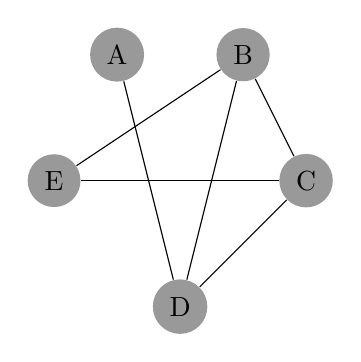
\begin{tikzpicture}
  [scale=.8,auto=left,
   every node/.style={circle,fill=black!40},
   0/.style={fill=red!50},
   1/.style={fill=blue!50},
   2/.style={fill=green!50},
   3/.style={fill=yellow!50},
   4/.style={fill=purple!50}]
  
  \node (A) at (2,4) {A};
  \node (B) at (4,4) {B};
  \node (C) at (5,2) {C};
  \node (D) at (3,0) {D};
  \node (E) at (1,2) {E};

  \foreach \from/\to in {A/D,B/C,B/E,C/E,D/B,C/D}
    \draw (\from) -- (\to);
\end{tikzpicture}



\subsubsection{Krok 0}

Graf:

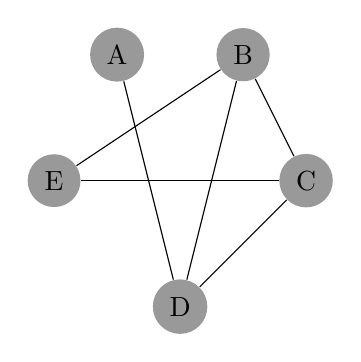
\begin{tikzpicture}
  [scale=.8,auto=left,
   every node/.style={circle,fill=black!40},
   0/.style={fill=red!50},
   1/.style={fill=blue!50},
   2/.style={fill=green!50},
   3/.style={fill=yellow!50},
   4/.style={fill=purple!50}]
  
  \node (A) at (2,4) {A};
  \node (B) at (4,4) {B};
  \node (C) at (5,2) {C};
  \node (D) at (3,0) {D};
  \node (E) at (1,2) {E};

  \foreach \from/\to in {A/D,B/C,B/E,C/E,D/B,C/D}
    \draw (\from) -- (\to);
\end{tikzpicture}

Lista tabu jest pusta.



\subsubsection{Krok 1}

Graf:

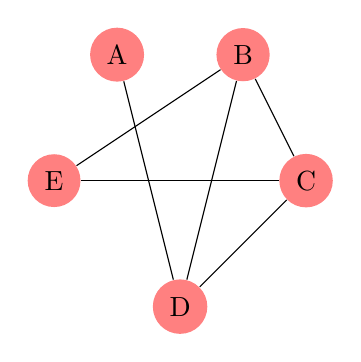
\begin{tikzpicture}
  [scale=.8,auto=left,
   every node/.style={circle,fill=black!40},
   0/.style={fill=red!50},
   1/.style={fill=blue!50},
   2/.style={fill=green!50},
   3/.style={fill=yellow!50},
   4/.style={fill=purple!50}]
  
  \node [0] (A) at (2,4) {A};
  \node [0] (B) at (4,4) {B};
  \node [0] (C) at (5,2) {C};
  \node [0] (D) at (3,0) {D};
  \node [0] (E) at (1,2) {E};

  \foreach \from/\to in {A/D,B/C,B/E,C/E,D/B,C/D}
    \draw (\from) -- (\to);
\end{tikzpicture}

Lista tabu:

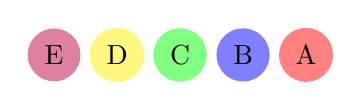
\begin{tikzpicture}
  [scale=.8,auto=left,
   every node/.style={circle,fill=black!40},
   0/.style={fill=red!50},
   1/.style={fill=blue!50},
   2/.style={fill=green!50},
   3/.style={fill=yellow!50},
   4/.style={fill=purple!50}]
  
  \node [0] (A) at (0,0) {A};
  \node [1] (B) at (-1,0) {B};
  \node [2] (C) at (-2,0) {C};
  \node [3] (D) at (-3,0) {D};
  \node [4] (E) at (-4,0) {E};
\end{tikzpicture}